\section{Full-coil validation and transfer to the spatial rod}
\label{sec:physical-results}

\subsection{Energy-consistent forces can still invalidate an affine plant}
Independent checks establish consistency of the coil interface before evaluating control. For the final coil kernel and force allocator, geometric virtual work and differentiated magnetic energy differ by $4.44\times10^{-16}$ in the canonical force norm. Twelve-direction energy differences with perturbations $2\times10^{-6}$ and $10^{-6}$ give errors $3.70\times10^{-10}$ and $7.04\times10^{-10}$. An axial circular-loop closed form checks absolute SI units to relative error $3.90\times10^{-16}$; sampled divergence and curl defects are below $1.58\times10^{-17}$\,T\,m$^{-1}$. Changing loop quadrature from 128 to 256 to 512 points changes the force by at most $3.69\times10^{-16}$. These local floating-point checks support the implemented energy/force interface, without certifying a continuous operating domain.

The resulting full-coil force nevertheless differs substantially from the affine field having the same origin field, gradient, and total currents. Table~\ref{tab:coil-quadrature} and Figure~\ref{fig:coil} compare the same physical Ritz coefficients, pulling all forces back to the 20-cell canonical coordinates. The approximately 98.6\% relative discrepancy persists with spatial refinement. It is therefore not explained by loop integration error or solely by the single magnetic point of the coarse geometry. Absolute full-force differences remain $0.00586672$ and $0.00145763$ between consecutive spatial grids; the 20-cell approximation is not spatially converged. The rank increase also shows why quadrature-dependent reachability must be measured, rather than inferred from the number of current channels.

\begin{table}[t]
\centering
\caption{Common-configuration coil-force and reachability diagnostics. Relative force error is $\|F_{\rm full}-F_{\rm affine}\|/\|F_{\rm full}\|$; current-port rank uses relative threshold $10^{-8}$.}
\label{tab:coil-quadrature}
\begin{tabular}{@{}rrrr@{}}
\toprule
\shortstack{Spatial\\cells} & \shortstack{Magnetic\\points} & \shortstack{Relative\\force error} & \shortstack{Rank of\\$G_I$}\\
\midrule
20 & 1 & 0.985235663 & 5\\
40 & 2 & 0.985978752 & 7\\
80 & 4 & 0.986182968 & 7\\
\bottomrule
\end{tabular}
\end{table}

\begin{figure*}[t]
\centering
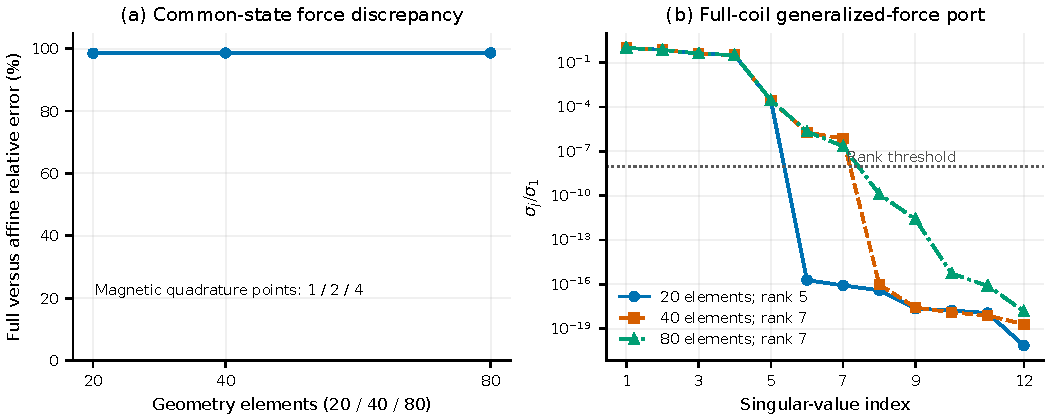
\includegraphics[width=\textwidth]{../figures/coil.pdf}
\caption{Full-coil force discrepancy and normalized current-port singular values at the same physical Ritz coefficients $q$ for 20/40/80 spatial quadrature cells. All forces and ports use the common 20-cell canonical basis. Magnetic quadrature has 1/2/4 active points. The persistent approximately 98.6\% affine discrepancy and numerical ranks 5/7/7 at relative threshold $10^{-8}$ preclude interpreting twelve coil channels as twelve independent generalized forces.}
\label{fig:coil}
\end{figure*}

For $d=0.2P_0$ and a $0.1$\,ms allocation interval, the orthogonal unreachable residual is $2.65530\times10^{-4}$ and the constrained residual is $4.01583\times10^{-4}$, with the 20\,A\,s$^{-1}$ limit active. Increasing this target by factors 10 and 100 gives constrained residuals $0.00500641$ and $0.07305644$. Correct feedback differentiation has directional finite-difference error $2.40\times10^{-9}$; differentiating the composed Hamiltonian instead changes the field by $5.47301$, while freezing feedback omits a Jacobian contribution of spectral norm $12.56491$. These are distinct implementation errors with direct consequences for an implicit closed-loop update.

\subsection{Actual constrained trajectories and their resolution limit}
The controlled trajectories are independently integrated from the same $z_0=\operatorname{initial\_state}(0.01)$, total bias, material, gain, and constraints. With $\gamma=0.2$, eight control updates cover $\tau\in[0,0.004]$, or $0.89733794$\,ms. One or two RK4 substeps per update give 8- and 16-step grids. Each branch evaluates its own feedback and actual plant force; an affine trajectory is not reused as a full-field trajectory.

The full-plant/full-controller and affine-plant/affine-controller trajectories differ by $3.90705\times10^{-4}$ in maximum canonical state norm. Their coarse/fine differences are approximately $7.22\times10^{-8}$, so the plant approximation has a resolved effect. On the full plant, however, replacing the full controller with its affine counterpart changes the trajectory by only $7.17555\times10^{-8}$. This window does not resolve a performance benefit from the full-field controller design. All four branches, including force compensation, have total and mechanical energy--work residual magnitudes near $6.25\times10^{-11}$ on the fine grid. The largest sampled magnetic-point field and gradient are $0.501325$\,mT and $0.00431404$\,T\,m$^{-1}$. Force compensation reaches 20\,A\,s$^{-1}$, but leaves a maximum force residual about $4.01416\times10^{-4}$.

The final allocator starts the force objective from an independently verified feasible previous current. Its rerun changes the earlier successful compensation trajectory by at most $1.17\times10^{-12}$ and currents by $6.51\times10^{-10}$\,A. This agreement does not establish identical derivatives of the optimization algorithm. Recomputed 36-dimensional sampled maps with exactly matched initial bias have numerical ranks 28 and 36 for collocated projection and force compensation, respectively. Their condition numbers are $5.43\times10^{18}$ and $2.09\times10^5$ in the stated canonical/current coordinates. Mechanical-block defects relative to $K_0$ are $3.22749\times10^{-3}$ and $1.03008\times10^{-4}$. The force-allocation Jacobian changes by $1.77112\times10^{-4}$ between versions, chiefly in the current-output block, despite a terminal mechanical-state difference of only $1.04\times10^{-14}$. Thus successful feasible allocation and nearly identical trajectories do not establish a smooth, invertible, or symplectic sampled map.

\subsection{Environmental transfer: feasible execution without tracking improvement}
\begin{figure*}[t]
\centering
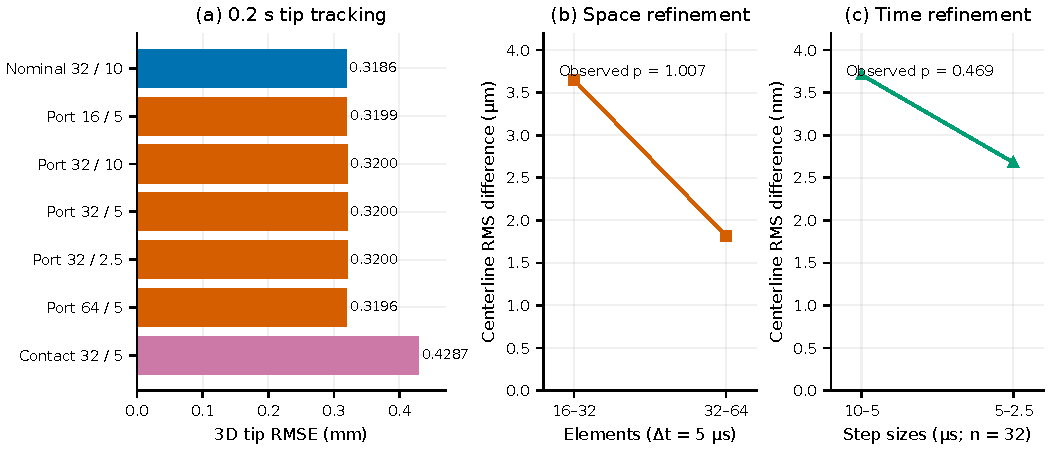
\includegraphics[width=\textwidth]{../figures/rod.pdf}
\caption{Spatial-rod transfer over 0.2\,s. Labels in (a) give the number of elements and time step in microseconds; nominal and port control are fairly compared at 32 elements and 10\,$\mu$s. The contact case is a separate 1.6\,mm-radius lumen geometry, whereas all other cases use the nominal 3\,mm lumen. Panels (b,c) show adjacent centerline differences at common times and 129 reference-arclength points. Observed rates describe these numerical differences and do not establish exact PDE error or second-order temporal convergence.}
\label{fig:rod}
\end{figure*}
Seven spatial-rod runs use the full coil forces and the physical gain in \eqref{eq:port-units}, over $0.2$\,s from a straight stationary state and zero actual current. This horizon ends before the $0.3$\,s target ramp completes. The implementation uses PyElastica PositionVerlet with the environmental forces described above. On the matched 32-element, 10\,$\mu$s grid, nominal control gives tip RMSE $0.318558$\,mm and the added port feedback gives $0.320032$\,mm: tracking slightly worsens. The 32-element, 5\,$\mu$s port case gives $0.320033$\,mm, maximum current $1.67831$\,A, maximum slew 20\,A\,s$^{-1}$, zero ramp discontinuity, and zero recorded violation at the 387 fixed constraint samples. Saved-node full-field maxima are $0.279966$\,mT and $0.0223521$\,T\,m$^{-1}$. These finite samples do not certify a continuous workspace.

The nominal 3\,mm lumen does not activate contact. A separate 1.6\,mm-radius lumen starts without penetration and develops maximum penetration $61.6032$\,$\mu$m and total normal force $11.3524$\,$\mu$N, with RMSE $0.428689$\,mm. Figure~\ref{fig:rod} reports this stress case separately. Ideal incremental port power is nonpositive, but projected and ramp-start increments reach positive values $3.19262\times10^{-8}$ and $3.20376\times10^{-8}$\,W. The 32-element, 5\,$\mu$s mechanical energy--work residual is $1.24636\times10^{-14}$\,J. Accurate accounting therefore coexists with loss of the ideal executed-input dissipation guarantee.

The original allocator fallback introduced an approximately $0.133$\,A discrepancy and spoiled temporal refinement. The final implementation clips to the current boxes and analytically repairs along a segment from the previous feasible current; it retains all nonconverged optimizer statuses. The seven final cases have zero fallbacks, 99 repairs each, and one to four nonconverged statuses, so feasibility is not presented as proven optimality. Adjacent centerline RMS differences at 129 common arclength points are $3.64802/1.81514$\,$\mu$m for 16/32/64 elements and $3.70928/2.67939$\,nm for 10/5/2.5\,$\mu$s steps. Observed spatial and temporal rates are $1.00703$ and $0.469234$, respectively; neither exact PDE error nor second-order temporal convergence is established.

Finally, a separate 2\,ms conservative comparison matches initial state, material, and fixed currents while disabling flow, wall, gravity, and damping. ROM-to-rod centerline RMS differences increase from $7.85933$ to $11.2030$ to $14.1690$\,nm across 16/32/64 elements; the corresponding tip RMS differences are $33.4755$, $65.6852$, and $86.4209$\,nm. Ritz truncation, shear/stretch restrictions, quadrature, and base-frame discretization remain distinct model errors. Its fixed currents also produce a full-rod gradient of $0.798394$\,T\,m$^{-1}$, exceeding the $0.03$\,T\,m$^{-1}$ limit. This diagnostic is not a feasible navigation result or a converged ROM error certificate.
